\chapter{Appendix}

\section{Detailed Transparency Report and DNS Abuse Mitigation by Cloudflare}
\label{app:cloudfare}


\begin{itemize}
    \item \textbf{Abuse Reports and Actions Taken}
    \begin{enumerate}
        \item Handling Abuse Reports: Among many other DNS abuses, phising, malware, and copyright infringements are most common at 
        \item Termination of Services: 
        \begin{itemize}
            \item Suspended Accounts and Dom: In the last half of 2022, Cloudflare claims to be committed to suspending 206 accounts and 530 domains that have proof to host content for Child Sexual Abuse Material (CSAM).
        \end{itemize}
        \item  Uniform Domain Name Dispute Resolution Policy (UDRP) Requests: Approximately 21 UDRP requests were handled in the latter half of 2022, which shows that Cloudflare is quite serious about resolving domain disputes amicably.
        \end{enumerate}
    \item \textbf{Law Enforcement and Legal Compliance}
    \begin{enumerate}
        \item Legal Sufficiency Review: Cloudflare will respond only to requests of this kind that meet a legal requirement or exemplary cases. In the sphere of law enforcement, there are court orders and subpoenas.
        \item International Privacy Laws: The company will not allow a state to demand a data reach if the legatees of this state contradict such an approach to privacy dictated by the outside state to Cloudflare. This policy highlights the adherence of Cloudflare to previous and subsequent points of the legal framework.
        \item Emergency Disclosure Requests: In such cases, the company agrees to some level of disclosure when there is a formal requirement for legal follow-up.
        \item National Security Requests: The company claims that it only served transparently and open agencies and other organisations. That is why it appeals against national security orders that do not adhere to the purpose of transparent informatics company performance.
        \item International Data Requests: Respond to foreign government requests on US legal standard cases or case evaluations.
    \end{enumerate}
    \item \textbf{Mitigation of DNS Abuse}
    \begin{enumerate}
        \item Public Reporting and Transparency: Cloudflare publicly reports and discloses these triggers of abuse, their kinds and quantity, to be able to maintain transparency in the relation of trust that allows ant-abuse to exist. 
        \item Law Enforcement Cooperation: Continue your partnerships with law enforcement, ensuring that everything you do is justified from a legal perspective, particularly with respect to DNS abuse.
        \item Challenges to Mitigating DNS Abuse: It is difficult to find a proper balance between the role of each side in defending legal interests and allowing collaborative measures to be accountable for DNS commitment. 
        \item Efficiency of efforts: Even with those complications, Cloudflare efficiently mitigates abuse by facilitating root cause solutions and market factor multitude.
    \end{enumerate}
    \item \textbf{Proposals for Future Enhancements}
    \begin{enumerate}
    \item Stakeholder Cooperation: Coordinated law enforcement in service delivery and other roles. Formal collaboration with international organisations and agencies. 
    \item Advances in Abuse Detection: The organisation has also developed plans to invest in advanced technologies and machine learning to improve abuse detection and response times. 
    \item Transparency Reporting: The organisation has also assured the community of its commitment to further increase the frequency and level of detail in transparency reports this year, describing more clearly the nature and mitigation of DNS abuse.
    \item User Education and Awareness: The organisation has also committed to developing and, more importantly, distributing educational materials aimed at increasing user awareness of the risks related to cybersecurity and DNS abuse. 
    \item Policy and Legal Reforms: Because there is likely to be a conflict between privacy laws and external privacy laws, the solution also suggested two law enforcement demands, proposing that participants engage in advocating changes in the resolution of the arising conflict. 
    \item Multi-stakeholder Feedback Mechanism: developed and proposed to the Executive Board for adoption and implementation, which outlines feedback mechanisms that shall include input from users, civil societies, and other stakeholders. This feedback shall form the organisational foundation for improvement and policy formulation.
    \end{enumerate}
        
\end{itemize}





\section{Presentation Slides}

\begin{figure}[H]
  \centering
  \begin{subfigure}[b]{0.55\linewidth}
    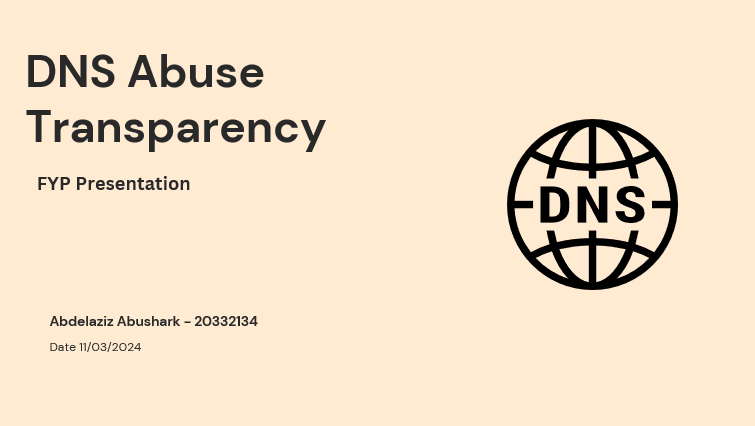
\includegraphics[width=\linewidth]{appendix/PRE1.png}
    \label{fig:left}
  \end{subfigure}
  \hfill % adds horizontal space between the figures
  \begin{subfigure}[b]{0.55\linewidth}
    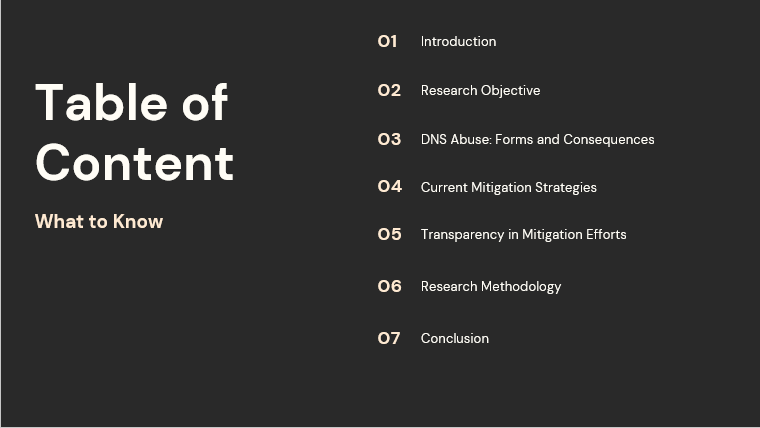
\includegraphics[width=\linewidth]{appendix/PRE2.png}
    \label{fig:right}
  \end{subfigure}
  \label{fig:images}
\end{figure}

\begin{figure}[H]
  \centering
  \begin{subfigure}[b]{0.55\textwidth}
    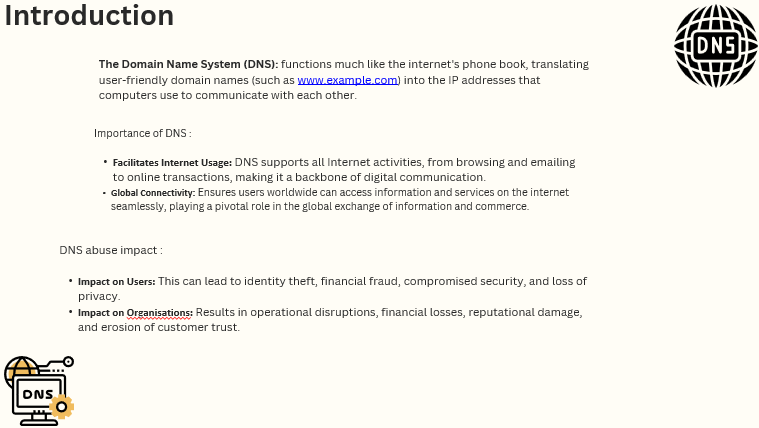
\includegraphics[width=\textwidth]{appendix/pre3.png}
    \label{fig:left}
  \end{subfigure}
  \hfill % adds horizontal space between the figures
  \begin{subfigure}[b]{0.55\textwidth}
    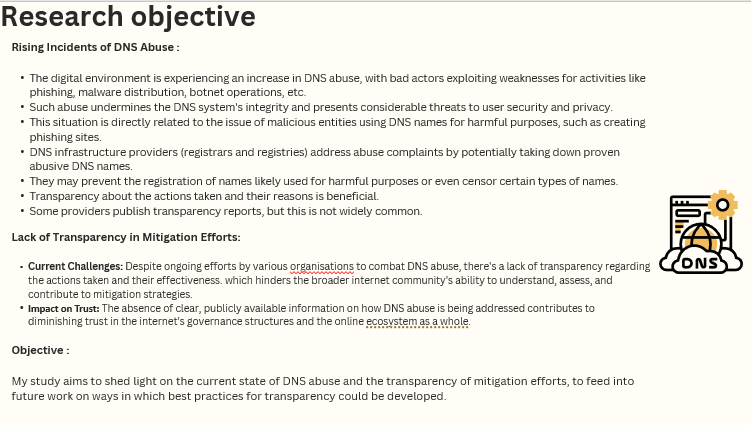
\includegraphics[width=\textwidth]{appendix/pre4.png}
    \label{fig:right}
  \end{subfigure}
  \label{fig:images}
\end{figure}

\begin{figure}[H]
  \centering
  \begin{subfigure}[b]{0.55\textwidth}
    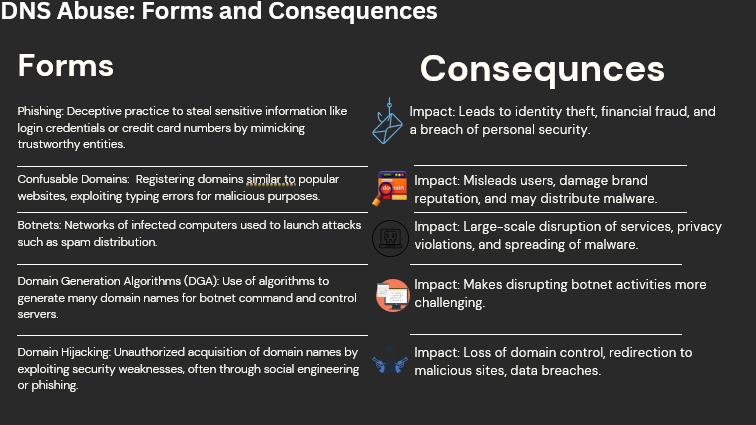
\includegraphics[width=\textwidth]{appendix/pre5.png}
    \label{fig:left}
  \end{subfigure}
  \hfill % adds horizontal space between the figures
  \begin{subfigure}[b]{0.55\textwidth}
    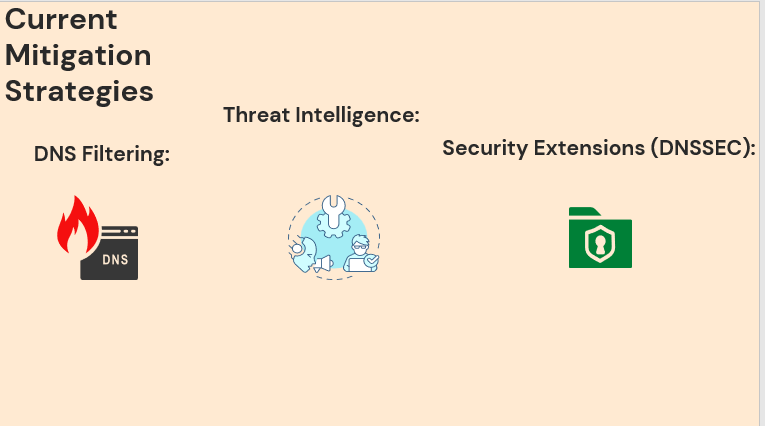
\includegraphics[width=\textwidth]{appendix/pre6.png}
    \label{fig:right}
  \end{subfigure}
  \label{fig:images}
\end{figure}

\begin{figure}[H]
  \centering
  \begin{subfigure}[b]{0.55\textwidth}
    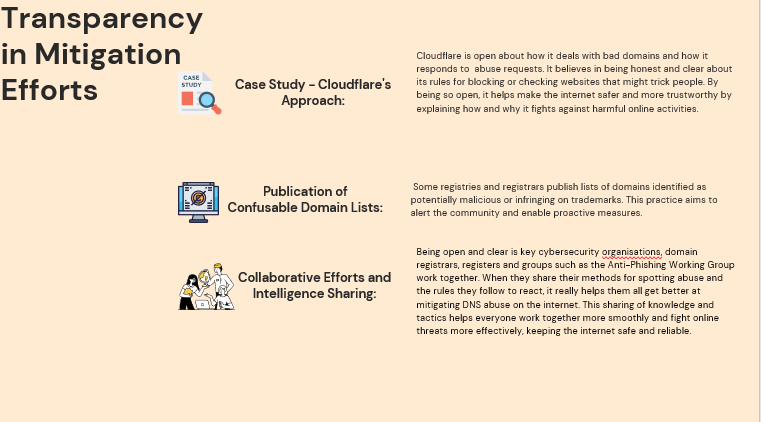
\includegraphics[width=\textwidth]{appendix/pre7.png}
    \label{fig:left}
  \end{subfigure}
  \hfill % adds horizontal space between the figures
  \begin{subfigure}[b]{0.55\textwidth}
    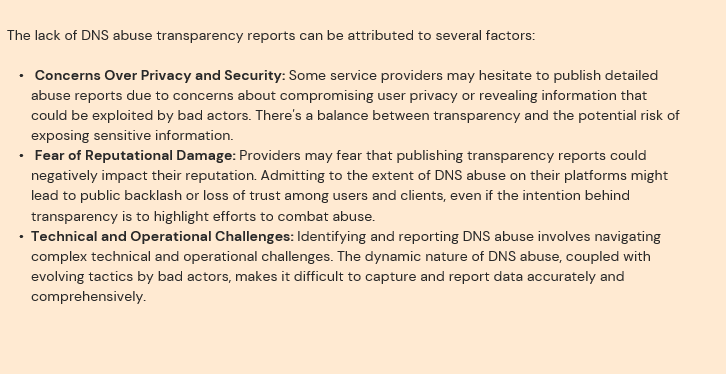
\includegraphics[width=\textwidth]{appendix/pre8.png}
    \label{fig:right}
  \end{subfigure}
  \label{fig:images}
\end{figure}

\begin{figure}[H]
  \centering
  \begin{subfigure}[b]{0.55\textwidth}
    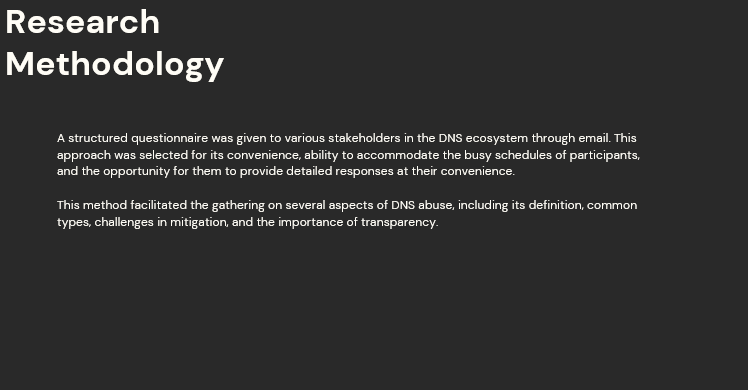
\includegraphics[width=\textwidth]{appendix/pre9.png}
    \label{fig:left}
  \end{subfigure}
  \hfill % adds horizontal space between the figures
  \begin{subfigure}[b]{0.55\textwidth}
    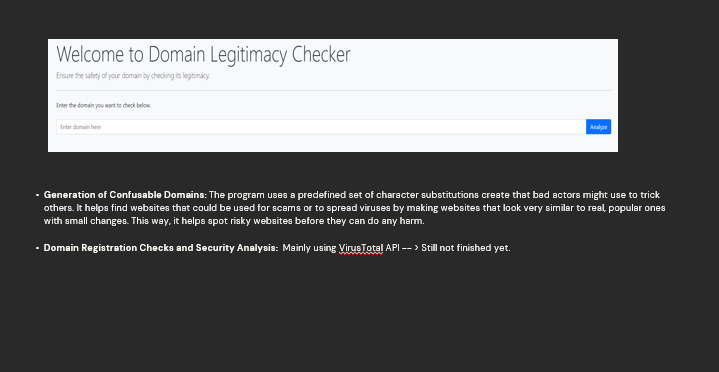
\includegraphics[width=\textwidth]{appendix/pre10.png}
    \label{fig:right}
  \end{subfigure}
  \label{fig:images}
\end{figure}

\begin{figure}[h]
    \centering
    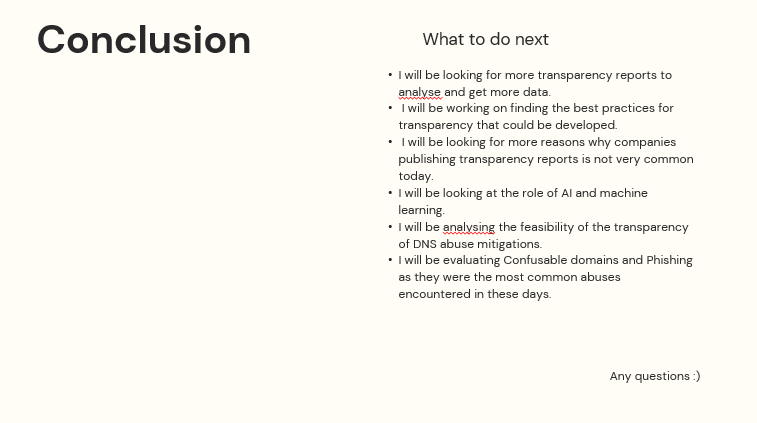
\includegraphics[width=0.55\linewidth]{appendix/pre11.png}
    \label{fig:lol}
\end{figure}